\documentclass[../main.tex]{subfiles}
\graphicspath{{\subfix{../../images/}}}

\begin{document}

A computer without an operating system is like a human without a soul. Without an OS installed on your computer, it would be no more than a fancy metal/plastic brick with silicon in it. 

\begin{figure}[H]
    \centering
    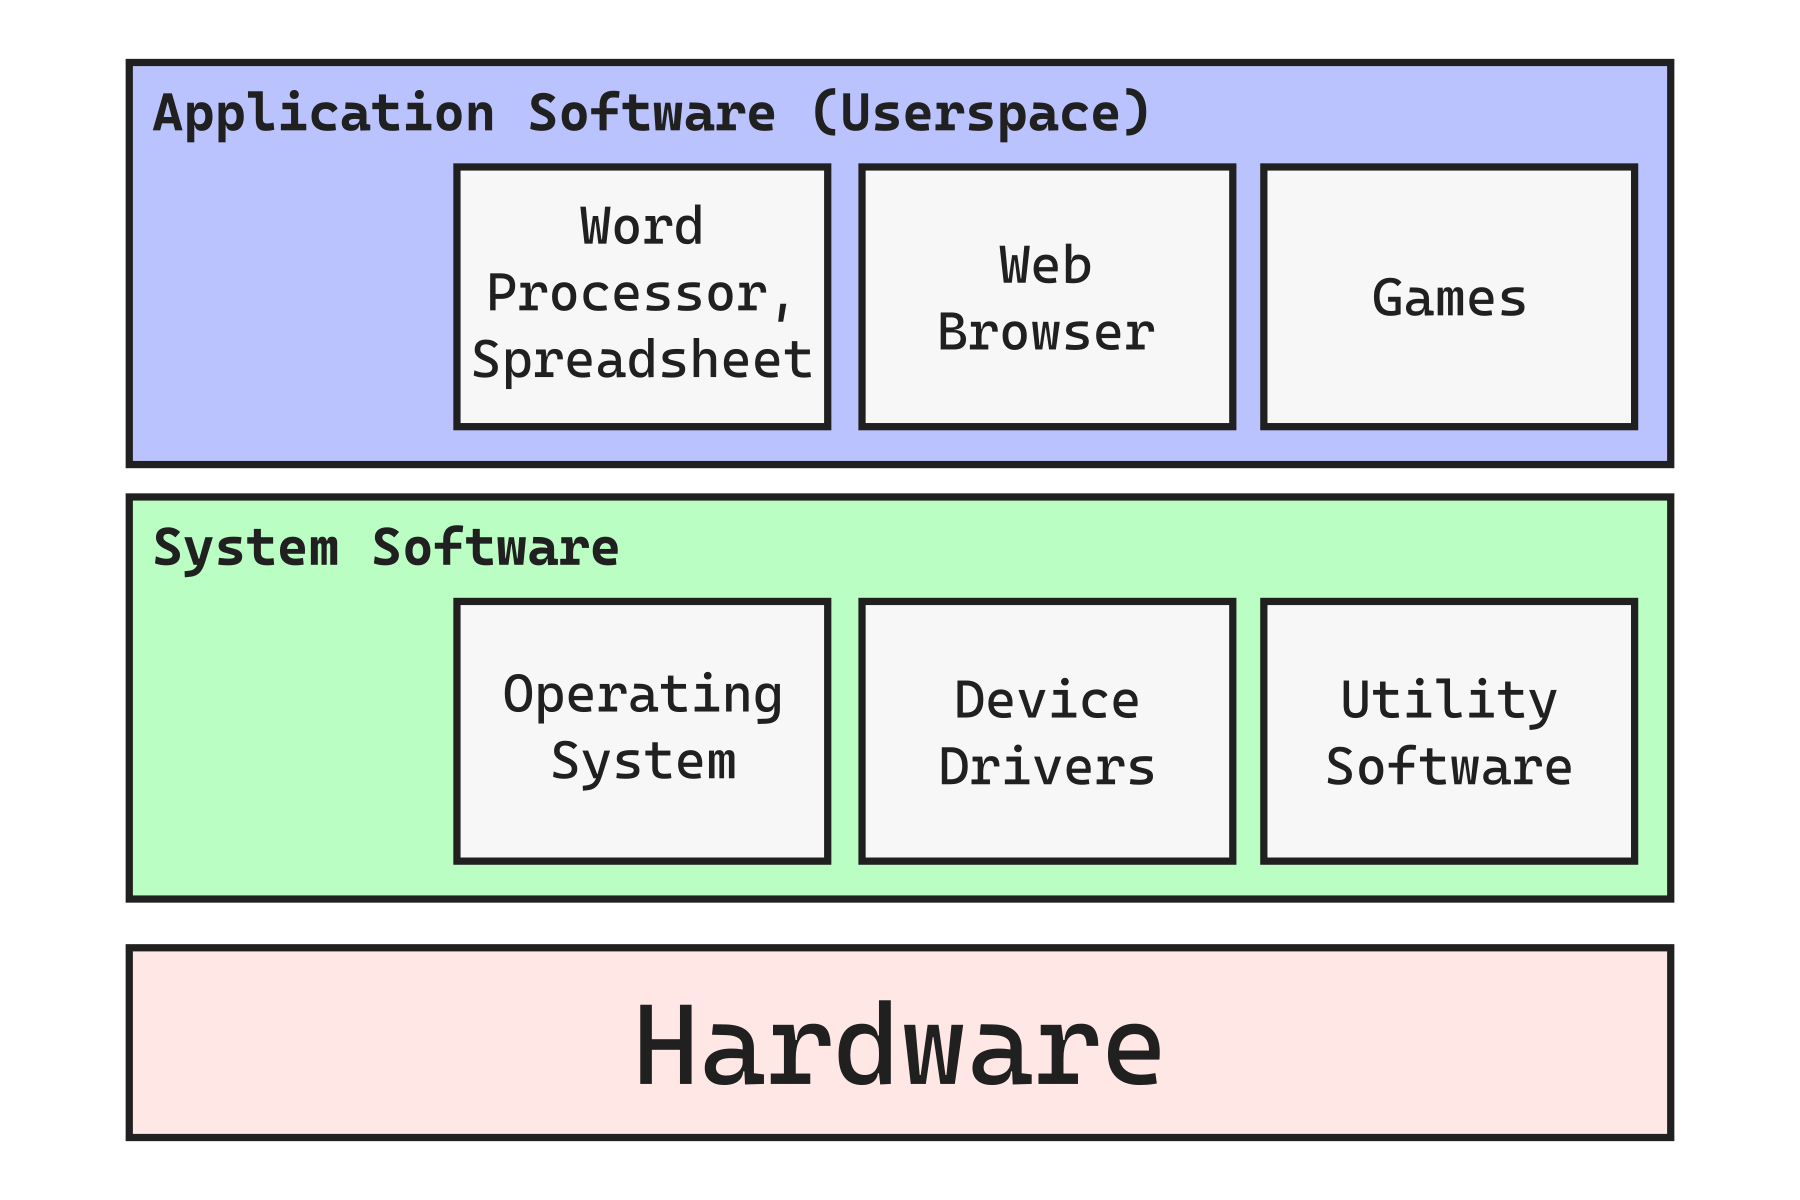
\includegraphics[width=0.85\textwidth]{software_stack.png}
    \caption{A very simplified software stack that Cambridge expects you to know.}
    \label{fig:software_stack}
\end{figure}

Figure \ref{fig:software_stack} shows the software that exists on your computer. All of this is stored in secondary storage on your boot device.

\subsection{The OS and System Software}

The operating system itself is a large set of programs that mainly run directly on the CPU, that gives the user an inteface to interact with the computer and connected devices, along with a mechanism to run programs, among others. The tasks that the OS carries out include:

\begin{enumerate}
    \item Loads device drivers for hardware and creates abstractions for application and utility software.
    \item Handles interrupts
    \item Creates and manages virtual memory (see section \ref{3:sec:virtmem}) for application and utility software
    \item Manages all files, including system files, files used by applications/programs and your files.
    \item Allows for multitasking
    \item Manages Hardware Peripherals
    \item Manages user accounts and their permissions on the computer.
    \item Provides a Human-Computer Interface (HCI)
    \item Provides Mouse/Keyboard input.
\end{enumerate}

Major Operating Systems include Microsoft Windows, Apple's macOS, Linux (GNU/Linux), and the *BSD family, among others. This is the reason why the interface you get when you use a Lenovo laptop, for example is different from if you use a Macintosh; the operating systems they use is different.

The kernel is simply a part of the operating system that creates the abstractions for hardware, so that userspace software can interact with it. On the list provided previously, items 1-5 is handled by the operating system, and the rest through special system software that is commonly grouped together with the OS. 

\subsubsection{Device Drivers}

Device Drivers, or just Drivers are pieces of software that enables hardware devices to communicate with the rest of the operating system. These drivers are what makes your devices, like your keyboard, mouse, monitor, camera, and even storage devices to function correctly. All devices that connect to your computer have drivers. 

In more complex terms, they are abstractions of the hardware and the raw electrical interfaces they provide for software written in higher-level languages to interact with.

\subsubsection{Multitasking}

Multitasking allows computers to carry out more than one task at a time. Each task is referred to as a \emph{process} (plural: processes). All of these processes at the end of the day share their resources with every other process (therefore the rest of the computer). A process on your computer could be the process drawing website content to your screen in your web browser, and another being your music player.

However, processes can clash, i.e. they request to be run at the exact same time. The CPU simply cannot run more than one instruction at the same time; even on multi-core processors they share one set of buses. Therefore, the CPU must do the following:

\begin{itemize}
    \item processes are allocated the computer's attention for a specific time.
    \item The process can be interrupted while it is running.
    \item The process is given a priority. Processes with more priority get more attention; they get more time to access the rest of the computer's resources. 
    \item Different processes are placed into attention at different times and they are alternated between (not at a specific rate, though).
\end{itemize}

This mechanism of swapping between processes very quickly gives one the impression processes run at the same time. This strategy is called preemptive multitasking. The technique of actually managing these resources is called \emph{scheduling}, it takes place within the operating system.

\subsubsection{Interrupts}
\label{4:sec:interrupts}

Interrupts are special signals that tells the CPU to immediately stop what it's doing to carry out something. There are two main types of interrupts, hardware and software interrupts.

\paragraph{Hardware Interrupts}

This is when I/O devices create data that the CPU must look at. This happens on:

\begin{itemize}
    \item Keyboard Presses
    \item Mouse movements
    \item Timer interrupts (for multitasking)
    \item Hardware failure (overheating)
\end{itemize}

To elaborate on \emph{timer interrupts}, this is the mechanism that tells the CPU to swap between different tasks.

\paragraph{Software Interrupts}

This is when software ran on the CPU itself generates interrupts. This happens in very specific cases, like:

\begin{itemize}
    \item Dividing by Zero
    \item Accessing memory out of bounds\footnote{Known as a segmentation fault. Since virtual memory is split into "containers" (see figure \ref{fig:virtmem}), when you access memory outside, the operating system disallows you to do so by sending an interrupt.}.
    \item Two processes trying to read/write to the same mory at the same time (known as a race condition).
    \item Extra: Asking the operating to do something (system call/syscall).
\end{itemize}

System calls, or syscalls is out of the syllabus, but is important to all software. In order for programs to do literally anything, like acessing I/O devices, reading and writing to disk, printing text, reading text and accessing the network, it has to ask the operating system\footnote{The kernel, to be more specific.} to do it, because it is the only thing that has the privelege of doing such things (security reasons). Doing this creates a type of interrupt that forces the CPU to give extra attention to it.

\paragraph{Buffers}

Buffers are just a general concept in programming that means a memory space used to put temporary data/collect data, only for it to be used and cleared later. In terms of OSes, buffers are used to maintain the state of programs before and after interrupts. Before an interrupt is called, the state of the CPU and virtual memory in the active process is saved to a buffer. After the interrupt, the memory is restored. The same happens when switching between processes for multitasking.

\paragraph{Servicing Interrupts}

When interrupts are received, they must be \emph{serviced}. Here are the procedures:

\begin{enumerate}
    \item The state of the Program Counter (see \ref{3:sec:vonneumann}), all registers and a portion of memory is saved.
    \item The interrupt service routine (ISR) is called, which is special code that is executed by loading the beginning of the code to the program counter. This makes the CPU start reading instructions from the ISR.
    \item The ISR decides what must happen from the type of the interrupt.
    \item The state of the registers, PC and memory is restored.
    \item Normal execution continues.
\end{enumerate}

Buffers and interrupts are typically used together in an OS to facilitate multitasking and interrupt handling. The textbook makes mention of a printer and how it uses buffers and interrupts. \textbf{The example is very oversimplified.}

Sending data to the printer from the CPU takes fractions of miliseconds. However, actually printing the data out can take around half a minute. If the CPU were to wait for this I/O operation to fully complete, the CPU would be stuck on one instruction telling the OS to print a single byte of data, meaning all other processes would not be able to run. The naïve solution would be to simply suspend the printing process and switch to another one, continuing multitasking. However, when the CPU returns to printing the document, it starts exactly where it left off, meaning it woult take even longer to print the document.

The solution is to save all the printing data into a print buffer, and instead of swapping between other processors and \emph{live-producing the bytes}, it simply reads a region of memory (the buffer) that has the data already prepared. This means that printing can happen at near-normal speed.

\subsubsection{Virtual Memory and Memory Management}
\label{4:sec:virtmem}

The operating system manages memory in the sense that it is responsible for creating virtual memory. Since the OS has direct access to memory (Direct Memory Access or DMA in the Linux kernel), and all I/O devices (the hard drive), it combines them in such a way that a pool of memory is made. When a process is created, a slice of that memory is made and is mapped to a full \emph{address space} for the process\footnote{Not all of the space is accessible; it is 64 bits as that is how wide the address bus is.}. This is known as memory mapping.

\begin{itemize}
    \item This is so that programs cannot access each other's memory, so that if a virus is on your computer, it cannot simply find your browser's memory space and read the passwords. 
    \item Processes also do not have to worry about accidentally overlapping with each other's space, causing interrupts.
    \item Memory can also be added and removed as needed. If the program needs more memory, it can take any piece of memory it needs from physical RAM or from the hard drive, and can tack itself onto the process's address space. This means that no drop of memory is wasted (ultimate rule in Computer Science).
\end{itemize}

This mechanism of dynamically adding/removing space for programs means that physical RAM does not have to be \emph{contiguous}, i.e. one next to each other. Instead it can look something like as follows:

\begin{figure}[H]
    \centering
    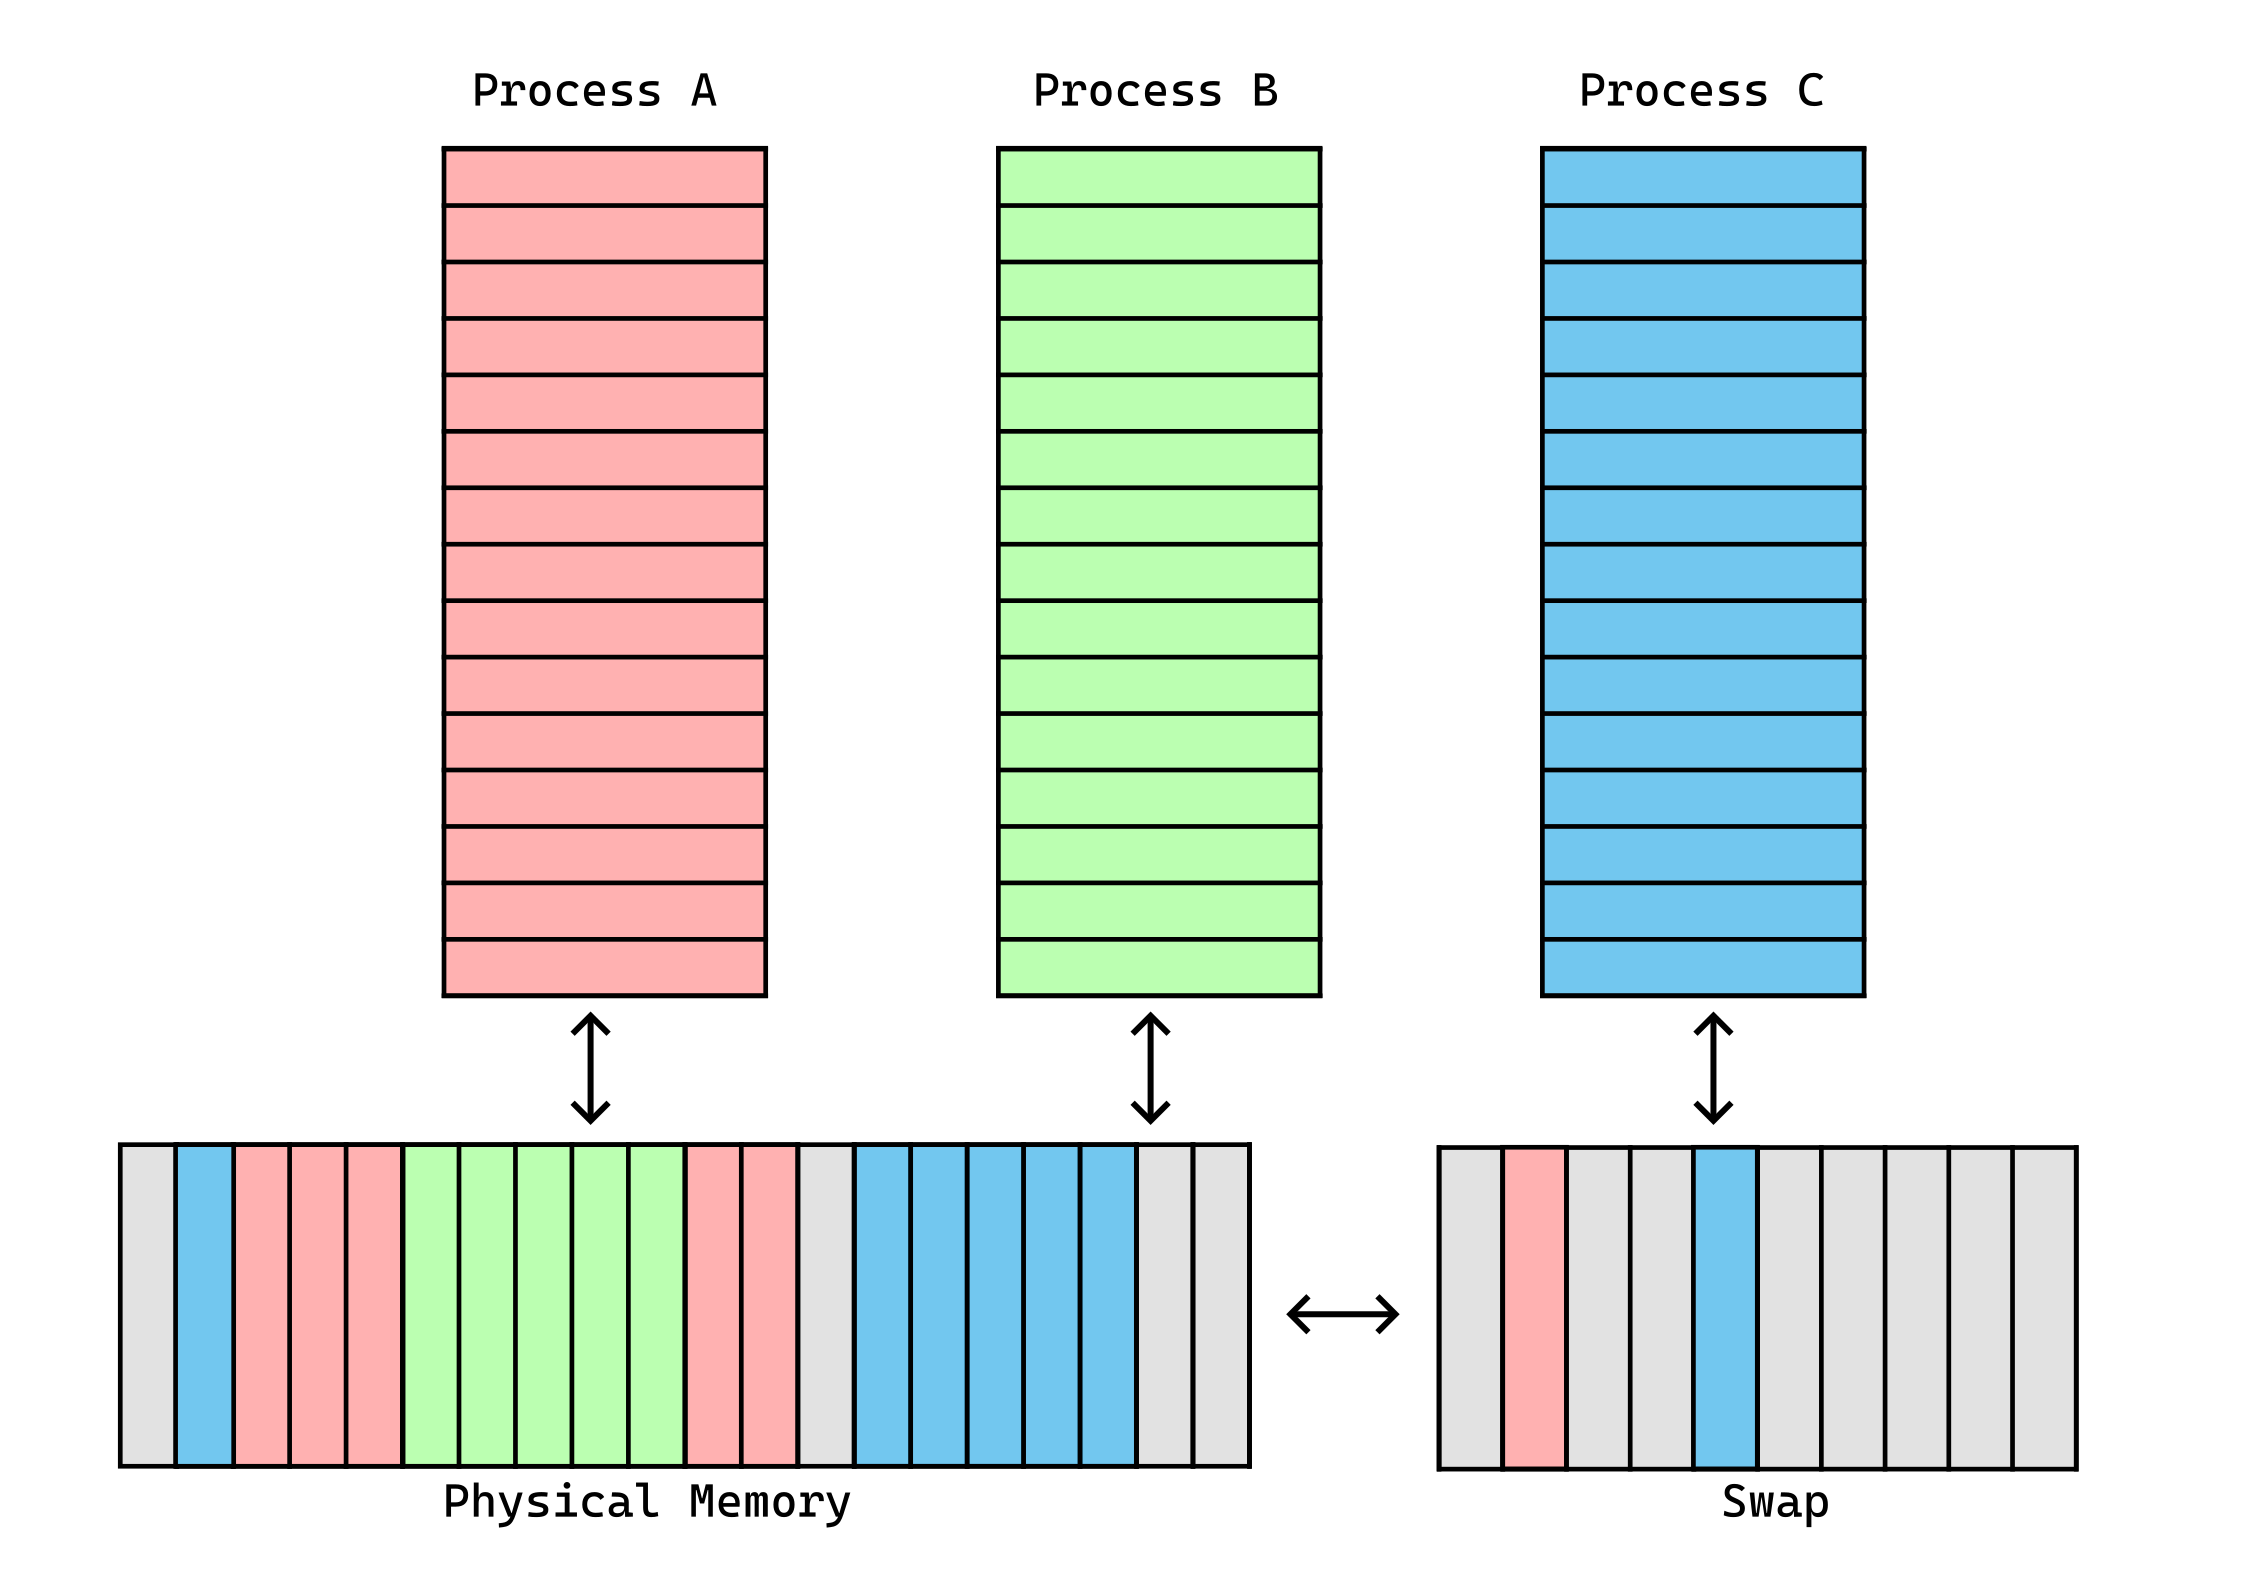
\includegraphics[width=0.8\textwidth]{memmap.png}
    \caption{Memory mapping.}
    \label{fig:memmap}
\end{figure}

NOTE: each chunk of memory is called a \textbf{page}. Each page is the same size as another.

\subsubsection{File Management}

File management in general is a complex topic, and due to time constraints it cannot be explained in as much detail as Virtual Memory. The general takeaways are:

\begin{enumerate}
    \item The hard drive is a hard slab of uselessness without a filesystem.
    \item Filesystems specify a set of rules that determine how the disk should be split into parts. Since files don't exist, nor do folders, the file system makes them exist. It specifies how files and folders should be laid out on disk so that the OS can interpret it as files and folders for its operation.
    \item The filesystem dictates things like file names and extensions (filename.pdf = filename is the file name and .pdf is the extension)
    \item Copying, moving, renaming, etc. is all handled by the OS through the filesystem.
    \item Filesystems can also have access control, meaning that different permissions (read, write, execute) can be set on files so that only specific users can can do the mentioned operations on them. As an example, teachers on a computer should be able to read and write to the folder of assessments, but students should only be able to read to the assessments.
    \item The operating system reads these files from the filesystem into memory for operation.
\end{enumerate}

\subsubsection{Hardware Peripheral Management}

The operating system interacts with hardware devices. In summary:

\begin{enumerate}
    \item The OS can communicate with all I/O devices through device drivers.
    \item Devices are actually represented as files on the filesystem (but not stored on the hard disk!). The kernel keeps the file open for itself to write to, and no other thing must interfere.
    \item The OS controls them by handling all the necessary interrupts (see section \ref{4:sec:interrupts}), and handles all buffers and queues.
\end{enumerate}

For more examples, refer to page 158 of the textbook.

\subsubsection{User Accounts and Permissions}

User accounts are a concept you should be familiar with. Accounts on a computer are not dissimilar from accounts on, say, Google; different users have different usernames and passwords on a computer system. This is useful for identifying different people, separating different users' data, and permissions management.

The OS manages all user accounts and sets up techniques to manage passwords and personal folders (home folders, what stores the desktop, documents, etc.) and manages who can access it. The OS creates different levels of privelege by segregating different users and granting them the ability to do different tasks based on their usernames and the user groups they are placed in. Some will have the privelege to write to the whole startup disk, while others only have privelege to write to their own home folder. Some will also have administrator priveleges while others will not.

This is not dissmilar to classroom management systems like the one at our school; teachers can create and set homework while we can only read them.

\subsubsection{Human-Computer Interfaces (HCI)}

HCI's allow the user to interact with the computer through an interface. There are 2 types of interfaces used in the modern day, \textbf{Command-line Interfaces (CLI)} and \textbf{Graphical User Interfaces (GUI)}. They allow the user to perform tasks the operating system is capable of doing (everything mentioned above), like launching programs, managing files and users. 

\paragraph{GUIs}

GUIs, or Graphical User Interfaces is the most common type of HCI out there.

\begin{figure}[H]
    \centering
    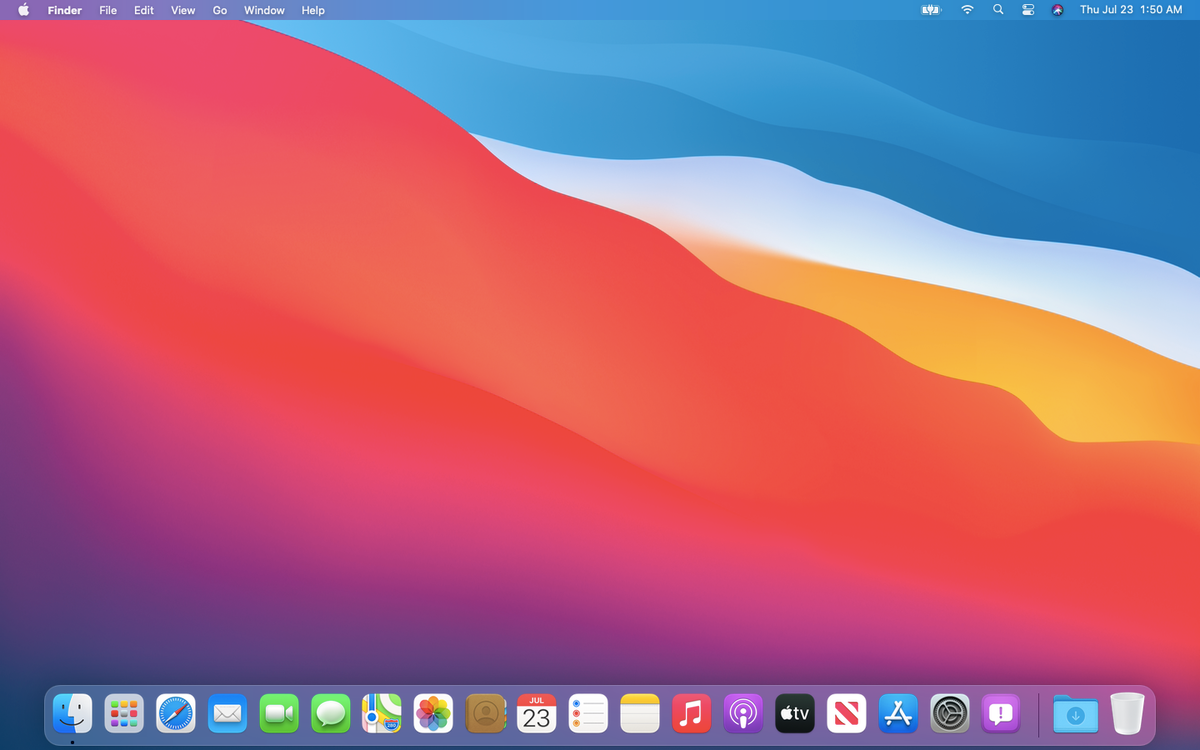
\includegraphics[width=0.7\textwidth]{macos11_desktop.png}
    \caption{The desktop of macOS 11 "Big Sur".}
    \label{fig:macos11:desktop}
\end{figure}

They usually use a group of technology called WIMP (Windows, Icons, Menus and Pointer) which includes all the elements mentioned previously to give you an interface with menus, windows, icons and a pointing device to navigate them. This was developed for use on personal computers (its origins are disputed) by several companies separately.

There are also post-WIMP interactions. This is used on both phones, tablets and some laptops with touchscreens here instead of using a pointer, the device uses less menus and more icons, buttons and gestures powered by the touchscreen to let the user navigate it. Both iOS and Android uses these. The most notable desktop OS that does not have post-WIMP interactions is macOS.

\paragraph{CLIs}

CLIs, or command line interfaces was the most prevalant HCI before GUIs were idealized. Even now, there are operating systems (Linux and BSDs) that allow the user to skip the WIMP stack and directly perform all tasks with a CLI.


\begin{figure}[H]
    \centering
    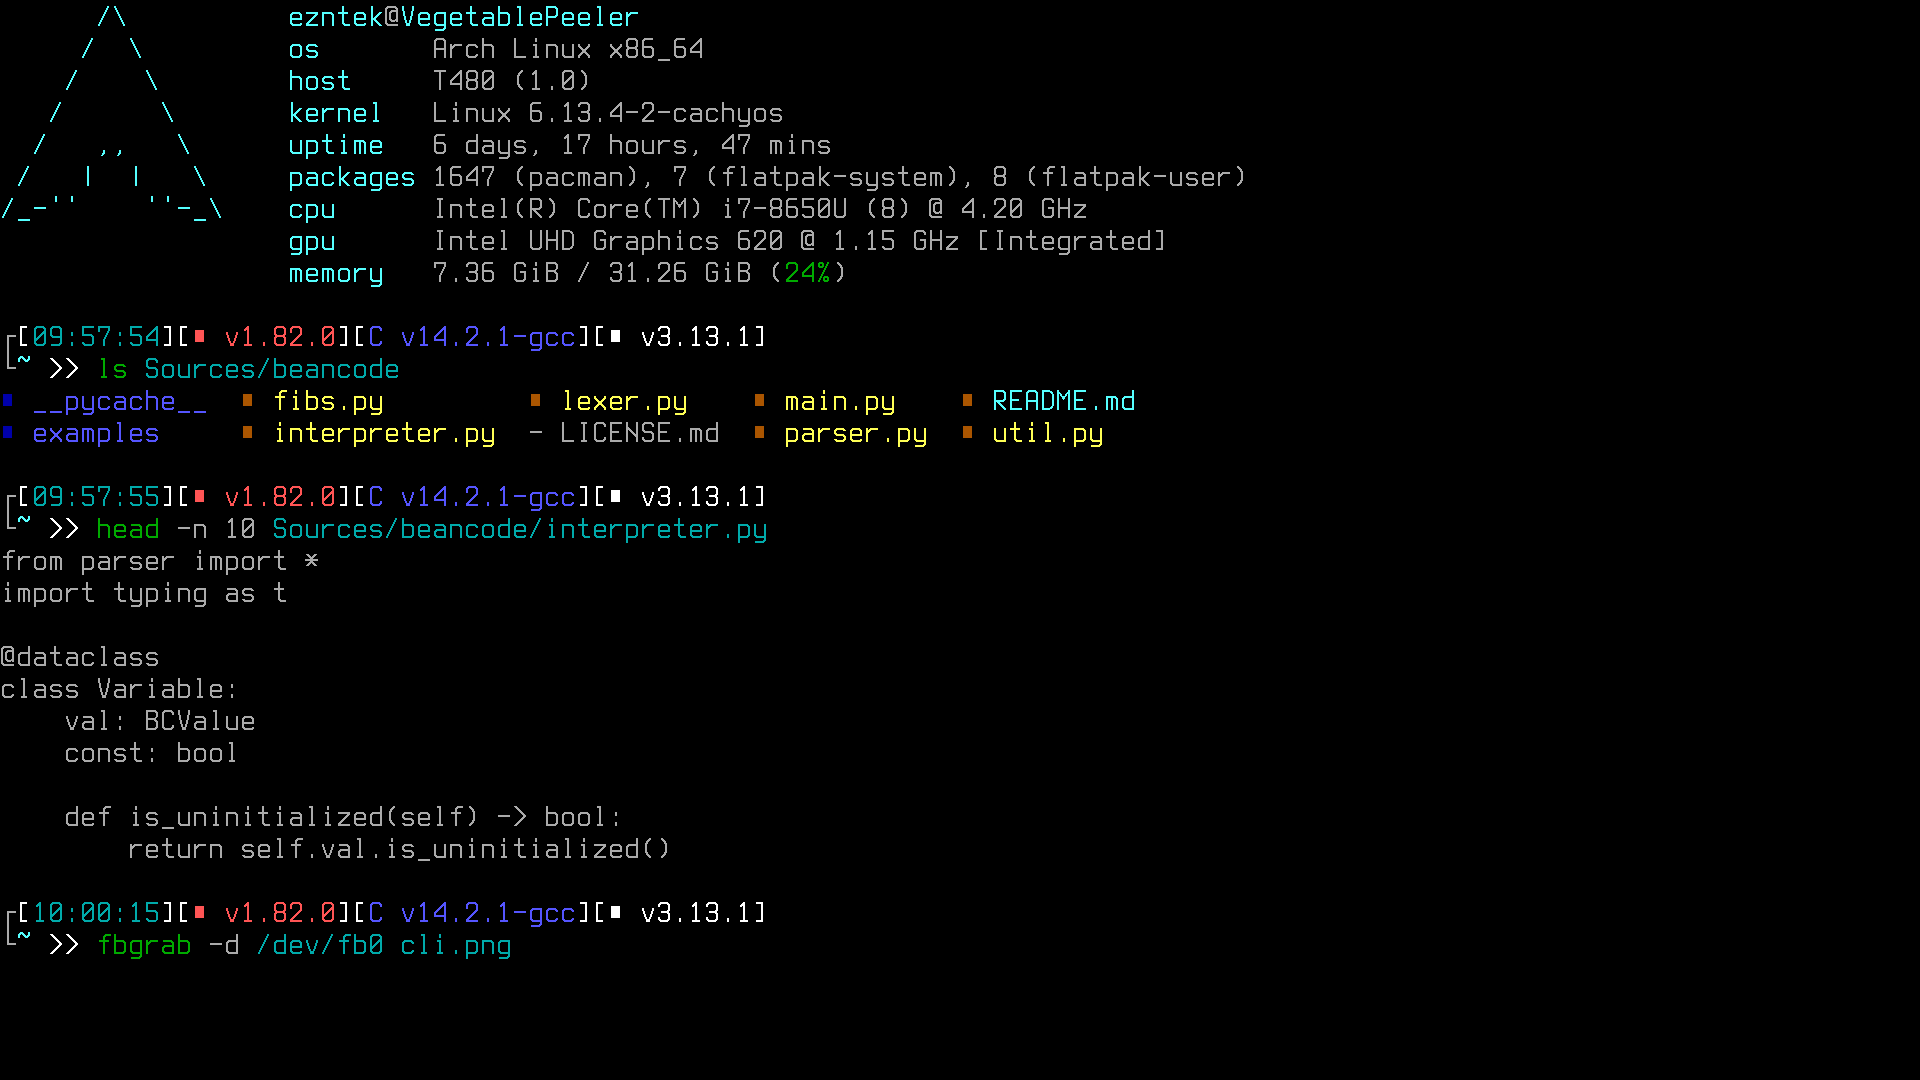
\includegraphics[width=0.9\textwidth]{cli.png}
    \caption{Linux in tty mode, meaning there is no GUI.}
    \label{fig:cli}
\end{figure}

CLIs, instead of GUIs do not make use of the mouse pointer, and there are no graphics, like windows and icons. Instead, you type comands into a \textbf{console} or \textbf{terminal} that perform very specific tasks, like making a directory with permissions or opening a text file and editing it.

Power users and programmers like you use CLIs, as you can directly communicate with the computer and operating system without needing to dig for menus here and there and constantly using the mouse to perform basic tasks. Instead, you only use the keyboard and type in the exact commands to do the exact things you must do all at once. CLIs also lets you automate complex tasks in the form of scripts, which run many commands one after another. You can use a \textbf{Terminal Emulator} to emulate a full CLI inside a window, like so:

\begin{figure}[H]
    \centering
    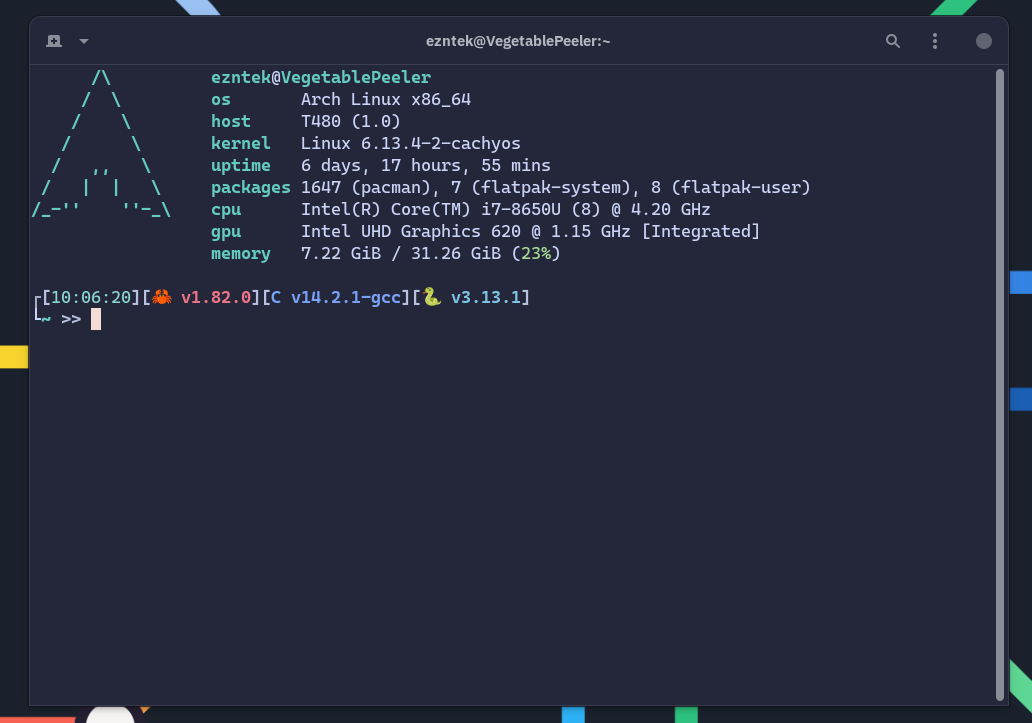
\includegraphics[width=0.7\textwidth]{terminal_emulator.png}
    \caption{A terminal emulator on Linux, which allows one to emulate a full terminal in a GUI.}
    \label{fig:terminal_emulator}
\end{figure}

\subsection{System Software}

What sits on top of the OS includes system software. These are pieces of software that allows hardware to run correctly, provides useful functions and allows the user to communicate with the computer. There are many examples of system software:

\begin{itemize}
    \item \textbf{Compilers, Interpreters and Linkers} will be covered in section \ref{4:sec:translators_compilers_and_interpreters}, but for now, know that this is what turns your code into machine code instructions that can be used in the fetch-decode-execute cycle.
    \item \textbf{Device Drivers} are pieces of software that directly run on the CPU and is a part of the kernel; that makes peripherals like your display, mouse and keyboard function correctly. They also provide an interface so that a userspace program can use it, like drawing to the display or reading the position of the mouse.
    \item \textbf{Other Examples} include antiviruses (provides protection against malicious software), defragmentation software (compacts space on HDDs), screenshot software, screensavers, your lock screen, a file browser, file backup software, etc.
\end{itemize}

For more detailed examples of system software, refer to the textbook in the corresponding section.


\end{document}
